\documentclass{article}
\usepackage{graphicx} % Required for inserting images
\usepackage{graphicx} % Required for inserting images
%\usepackage[left=0.5in, right=0.5in, top=0.5in, bottom=0.5in]{geometry}
%\usepackage[left=1.5cm, right=1cm, top=0.5cm, bottom=1.5cm]{geometry}
\usepackage[left=1.5cm, right=1.5cm, top=1cm, bottom=1.5cm]{geometry}
\usepackage{amsmath}
\usepackage{amssymb}
\usepackage{amsfonts}
\usepackage{amsthm}
\usepackage{ulem}
\usepackage{bm}
\usepackage{tikz}
\usepackage{enumitem}
\usepackage{enumerate}
\usetikzlibrary{shapes,backgrounds}
\usepackage{textcomp} % for \textdollar command
\usepackage{array}

\date{}

\begin{document}
\fontsize{13}{17} \selectfont %This is 13pt text with 16pt line spacing.
\setcounter{page}{2}

\begin{center}
    \textbf{SECTION A} \\

    \vspace{10pt}

    \textbf{Answer all questions. Write your answers in the spaces provided. } \\

    \vspace{10pt}

   \textbf{ In Section A draw a circle around the letter at the beginning of your choice to indicate your answer 
\includegraphics[width=0.6cm]{Exams/a_circle.png}. If you change your mind, put a line through the circle 
\includegraphics[width=0.6cm]{Exams/a_circle_crossed.png} and then draw a circle 
\includegraphics[width=0.6cm]{Exams/a_circle.png} around another choice. }
  
\end{center}

\vspace{5pt}

\begin{enumerate} 

% Q1
    \item Which of the following is the longest river in the world?
    
    (a)  Nile \\
    (b)  Amazon \\
    (c)  Mississippi \\ 
    (d)  Yangtze 

\hfill\raggedright (1 mark) 
\vspace{5pt}
\hline
\vspace{7pt}

% Q2
    \item The source of a river is:
    
    (a) Where the river meets the ocean \\
    (b)  The point where the river begins \\
    (c) The deepest part of the river \\
    (d) The widest part of the river 

\hfill\raggedright (1 mark) 
\vspace{5pt}
\hline
\vspace{7pt}

% Q3
    \item What is the function of a river delta?
    
    (a) It regulates the flow of the river \\
    (b) It is a source of drinking water \\
    (c) It forms a fertile area at the river's mouth \\
    (d) It prevents flooding along the riverbanks 

\hfill\raggedright (1 mark) 
\vspace{5pt}
\hline
\vspace{7pt} 

% Q4
    \item Which of the following is the longest river in the world?
    
    (a) Nile \\
    (b) Amazon \\
    (c) Mississippi \\
    (d) Yangtze 
    
\hfill\raggedright (1 mark) 
\vspace{5pt}
\hline
\vspace{7pt}

% Q5
    \item The source of a river is:
    
    (a) Where the river meets the ocean \\
    (b) The point where the river begins \\
    (c) The deepest part of the river \\
    (d) The widest part of the river 

\hfill\raggedright (1 mark) 
\vspace{5pt}
\hline
\vspace{7pt}

    \newpage

% Q6
    \item What is the mouth of a river?
    
    (a) Where the river meets the ocean \\
    (b) The point where the river begins \\
    (c) The deepest part of the river \\
    (d) The widest part of the river 

\hfill\raggedright (1 mark) 
\vspace{5pt}
\hline
\vspace{7pt} 

% Q7
    \item What is the primary purpose of a dam on a river?

    (a) Create a waterfall \\
    (b) Prevent river pollution \\
    (c) Control water flow and generate electricity \\
    (d) Increase river speed 

\hfill\raggedright (1 mark) 
\vspace{5pt}
\hline
\vspace{7pt}
   
% Q8
    \item In which continent is the Amazon River located?
    
    (a) Asia \\
    (b) Africa \\
    (c) South America \\
    (d) Australia 

\hfill\raggedright (1 mark) 
\vspace{5pt}
\hline
\vspace{7pt}

% Q9
    \item What is the largest river considering the amount of water it carries?
    
    (a) Amazon \\
    (b) Yangtze \\
    (c) Congo \\
    (d) Ganges 

\hfill\raggedright (1 mark) 
\vspace{5pt}
\hline
\vspace{7pt}

% Q10
    \item What is the primary source of energy that drives the hydrological cycle?
    
    (a) Wind energy \\
    (b) Solar energy \\
    (c) Geothermal energy \\
    (d) Hydroelectric energy 

\hfill\raggedright (1 mark) 
\vspace{5pt}
\hline
\vspace{7pt}

% Q11
    \item During which process of the hydrological cycle does water change from a liquid to a gas?
    
    (a) Evaporation \\
    (b) Condensation \\
    (c) Precipitation \\
    (d) Infiltration 

\hfill\raggedright (1 mark) 
\vspace{5pt}
\hline
\vspace{7pt}

\newpage

% Q12
    \item What is the term for the process by which plants release water vapor into the atmosphere?
    
    (a) Transpiration \\
    (b) Percolation \\
    (c) Saturation \\
    (d) Runoff 

\hfill\raggedright (1 mark) 
\vspace{5pt}
\hline
\vspace{7pt}

% Q13
    \item Which of the following is a form of precipitation?
    
    (a) Fog \\
    (b) Dew \\
    (c) Hail \\
    (d) All of the above 

\hfill\raggedright (1 mark) 
\vspace{5pt}
\hline
\vspace{7pt}

% Q14 
    \item What role do oceans play in the hydrological cycle?
    
    (a) Oceans only receive water, not release it. \\
    (b) Oceans release water vapor through precipitation. \\
    (c) Oceans absorb sunlight and regulate temperature. \\
    (d) Oceans have no impact on the hydrological cycle. 

\hfill\raggedright (1 mark) 
\vspace{5pt}
\hline
\vspace{7pt}

% Q15
    \item Which one is a major source of river pollution in cities?  

    (a) Industrial waste \\
    (b) Smoke \\
    (c) Farm chemicals   \\
    (d) Fertilizers 

\hfill\raggedright (1 mark) 
\vspace{5pt}
\hline
\vspace{7pt}

% Q16
    \item What is the term for the process of treating wastewater before it is released into rivers or other water bodies?
    
    (a) Desalination \\
    (b) Filtration \\
    (c) Aeration \\
    (d) Water purification 

\hfill\raggedright (1 mark) 
\vspace{5pt}
\hline
\vspace{7pt}

\newpage

  % Q17
    \item Which of the following is a sustainable practice for river management to prevent pollution?
    
    (a) Damming rivers to control water flow \\
    (b) Reducing the use of plastic and promoting recycling \\
    (c) Discharging untreated industrial waste into rivers \\
    (d) Increasing the release of warm water from power plan

\hfill\raggedright (1 mark) 
\vspace{5pt}
\hline
\vspace{7pt}

% Q18
\item Which one is NOT a common cause of river flooding?
    
    (a) Deforestation \\
    (b) Urbanization \\
    (c) Drought \\
    (d) Excessive precipitation 

\hfill\raggedright (1 mark) 
\vspace{5pt}
\hline
\vspace{7pt}

% 19
    \item How does construction contribute to flooding?
    
    (a) Buildings prevent water from getting into the ground. \\
    (b) Buildings reduce the speed of surface water flow. \\
    (c) Buildings reduce the risk of riverbank overflow. \\
    (d) Levees enhance groundwater flow. 

\hfill\raggedright (1 mark) 
\vspace{5pt}
\hline
\vspace{7pt}

% Q20
    \item What is a negative effect of large-scale dam construction for flood control?
    
    (a) Increased river flow \\
    (b) Habitat destruction \\
    (c) Erosion prevention \\
    (d) Improved water quality 

\hfill\raggedright (1 mark) 
\vspace{5pt}
\hline
\vspace{7pt}

\vspace{5pt}
\rule{\linewidth}{2pt} \\ 
\hfill\raggedright \textbf{TOTAL FOR SECTION A IS 20 MARKS} 
\vspace{5pt}

\newpage
% Section B

\begin{center}
\textbf{SECTION B} \\
\vspace{10pt}
\textbf{Answer all questions.}
\end{center}

% Q21
\item Use \textbf{arrows} to match the words on the left side and the descriptions on the right side.

% Table 2
\begin{table}[h]
    \centering
    \begin{tabular}{c@{\hspace{3cm}} c@{\hspace{3cm}} c} \\ \vspace{10pt}
        Mouth &  & A boundary between two drainage basins \\ \vspace{10pt}
        Confluence &  & A smaller river joining a bigger river \\ \vspace{10pt}
        Tributary &  & Where a tributary joins the main river \\ \vspace{10pt}
        Watershed &  & Where the river ends \\ \vspace{10pt}
    \end{tabular}
    %\caption{Match the words with their descriptions.}
    %\label{tab:matching}
\end{table}

\hfill\raggedright (4 marks) 
\vspace{5pt}
\hline
\vspace{7pt}

% Q22
\item Give \textbf{two} steps you would take to prevent river pollution
\vspace{10pt}

(i)\dotuline{\hspace{16cm}} \\
\vspace{7pt}
\quad \dotuline{\hspace{16cm}} \\
\vspace{7pt}

(ii)\dotuline{\hspace{16cm}} \\
\vspace{7pt}
\quad \dotuline{\hspace{16cm}} \\
\vspace{7pt}

\hfill\raggedright (2 marks) 
\vspace{5pt}
\hline
\vspace{7pt}

% Q23
\item The children in Frank's class chose their favourite fruit. Their answers are listed below. \\
\begin{center}
apple \hspace{1cm} orange \hspace{1cm} melon \hspace{1cm} apple \hspace{1cm} apple \\
melon \hspace{1cm} apple \hspace{1cm} orange \hspace{1cm} apple \hspace{1cm} orange \\
orange\hspace{1cm} peach \hspace{1cm} mango \hspace{1cm} melon \hspace{1cm} apple \\
apple \hspace{1cm} apple \hspace{1cm} peach \hspace{1cm} apple \hspace{1cm} melon \\
peach \hspace{1cm} apple \hspace{1cm} orange \hspace{1cm} apple \hspace{1cm} orange 
\end{center} 

(a) Complete a \textbf{tally chart} for this information. Melon has been done for you.

\begin{table}[h]
    \centering
    
    \begin{tabular}{|c@{\hspace{3cm}}|c@{\hspace{3cm}} |} \hline 
      Fruit & \rule[-8pt]{0pt}{22pt} Tallies  \\ \hline 
      Apple & \rule[-8pt]{0pt}{22pt} \\ \hline
      Orange & \rule[-8pt]{0pt}{22pt} \\ \hline
      Melon & \rule[-8pt]{0pt}{22pt}\vert \vert \vert \vert \\ \hline
      Peach & \rule[-8pt]{0pt}{22pt} \\ \hline
      Mango & \rule[-8pt]{0pt}{22pt} \\  
      \hline
    \end{tabular}
    %\caption{Caption}
    %\label{tab:my_label}
\end{table} 

\hfill\raggedright (2 marks) 
\vspace{5pt}
%\hline
%\vspace{3pt}

(b) Draw a \textbf{Bar Chart} to represent the information.
\vspace{20pt}
\begin{center}

\includegraphics[wiodth=12cm]{Exams/10_by_10_grid.png}
\end{center}

\vspace{20pt}

\hfill\raggedright (4 marks) 
\vspace{5pt}
\hline
\vspace{7pt}

% Q24
\item \quad Here are the marks that Chemutai got in her Geography tests.
\begin{center}
\( \displaystyle 29 \hspace{1cm} 24 \hspace{1cm} 26 \hspace{1cm} 25 \hspace{1cm} 25 \hspace{1cm} 25 \hspace{1cm} 28 \)  \\ 
\end{center}
(a) What is the mode of Chemutai’s marks?

\vspace{30pt}
\hspace{15cm} .......... 
\vspace{5pt}

\hfill\raggedright (1 mark) 
\vspace{5pt}
\hline
\vspace{7pt}

(b) What is the range in Chemutai’s marks?

\vspace{30pt}
\hspace{15cm} .......... 
\vspace{5pt}

\hfill\raggedright (1 mark) 
\vspace{5pt}
\hline
\vspace{7pt}

(c) What is the mean of Chemutai’s marks?

\vspace{100pt}
\hspace{15cm} .......... 
\vspace{5pt}

\hfill\raggedright (1 mark) 
\vspace{5pt}
\hline
\vspace{7pt}

(d) What is the median of Chemutai’s marks?

\vspace{120pt}
\hspace{15cm} .......... 
\vspace{5pt}

\hfill\raggedright (1 mark) 
\vspace{5pt}
\hline
\vspace{7pt}

% Q25
\item Use the map below to answer the questions that follow. 

\begin{center}
    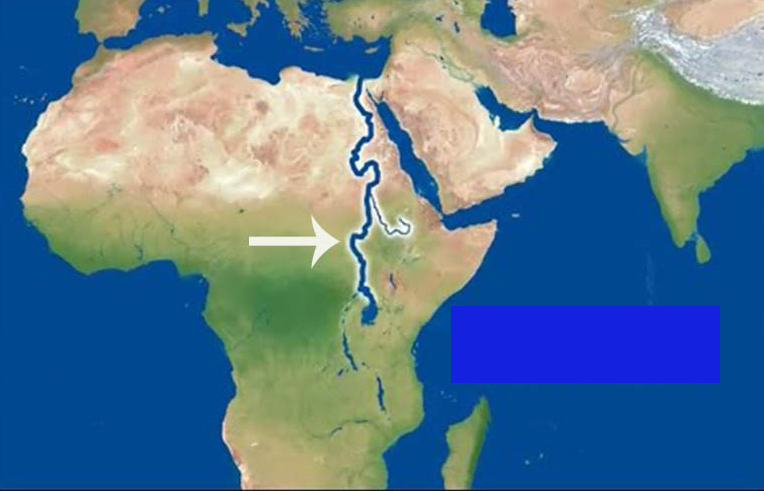
\includegraphics[width=12cm]{Exams/Nile_2.png}
\end{center}

(a) Identify the river shown by the arrow. \\ \vspace{10pt}

\dotuline{\hspace{16cm}} \\
\vspace{7pt}

\hfill\raggedright (1 mark) 
\vspace{5pt}
\hline
\vspace{3pt}

\newpage

(b) Outline \textbf{three} benefits provided by the river. \\
\vspace{15pt}

(i) \dotuline{\hspace{16.5cm}} \\
 \vspace{15pt}

\quad \dotuline{\hspace{16.5cm}} \\
\vspace{15pt}

(ii) \dotuline{\hspace{16.5cm}} \\
\vspace{15pt}

\quad \dotuline{\hspace{16.5cm}} \\
\vspace{15pt}

(iii) \dotuline{\hspace{16.5cm}} \\
\vspace{15pt}

\quad \dotuline{\hspace{16.5cm}} \\
\vspace{15pt}

\hfill\raggedright (3 marks) 
\vspace{5pt}
\hline
\vspace{7pt}

\vspace{5pt}
\rule{\linewidth}{2pt} \\ 
\hfill\raggedright \textbf{TOTAL FOR SECTION B IS 20 MARKS}  \\
\hfill\raggedright \textbf{TOTAL FOR PAPER IS 40 MARKS} \\
\vspace{90pt}

\hspace{8cm} \textbf{The End}


\end{enumerate}

\end{document}